\documentclass[twocolumn]{aastex62}

\usepackage{stix}
\usepackage{xspace}
\usepackage{hyperref}
\usepackage{todonotes}
\newcommand{\vdag}{(v)^\dagger}
\newcommand\aastex{AAS\TeX}
\newcommand\latex{La\TeX}
\newcommand{\mjup}{\ensuremath{M_\mathrm{Jup}}\xspace}
\newcommand{\teff}{\ensuremath{T_{\mathrm{eff}}}\xspace}
\newcommand{\logg}{\ensuremath{\log(g)}\xspace}
\graphicspath{{./}{figures/}}
\shorttitle{HD106906b Time Resolved Observations}
\shortauthors{Zhou et al.}

\begin{document}


\title{Cloud Atlas: High-precision time-resolved observations of exoplanet HD106906b}

\correspondingauthor{Yifan Zhou}
\email{yzhou@as.arizona.edu}

\author{Yifan Zhou}
\affil{Steward Observatory}

\author{D\'aniel Apai}
\affil{Steward Observatory}

\begin{abstract}
TBD
\end{abstract}

\keywords{}

\section{Introduction}

HD106906b is a $11\pm2$ \mjup  mass exoplanet \citep{Bailey2013} to a F5V type star. This system, at a distance of $103.3\pm0.4$ pc \citep{Gaia2016,Gaia2018}, is a member of the Lower Centaurus Crux association (99.8 membership probability based on BANYAN-$\Sigma$, \citealt{Gagne2018} ), which is a part of the Sco-Cen star forming region \citep[age: $15\pm3$ Myr][]{Pecaut2016}. The planet and the star has a wide angular separation of $7\arcsec.11\pm0\arcsec.03$\citep{Bailey2013}, corresponding to a projected distance of $734\pm4$ au.  HD106906b is among the most favorable exoplanets for atmospheric characterizations \citep[e.g., ]{Bailey2013,Kalas2015,Wu2016,Daemgen2017} due to its wide angular separation to its host and moderate brightness contrast.

Multi-wavelength photometry \citep{Bailey2013,Kalas2015,Wu2016} and spectroscopy \citep{Bailey2013, Daemgen2017} observations have been used to characterize HD106906b's atmosphere.  These studies agree on an effective temperature (\teff) of 1800~K and a spectral type classification of L2.5-3. Based on its triangle-shaped $H$-band spectrum, both \citet{Bailey2013, Daemgen2017} classified HD106906b as an intermediate- to low-surface gravity object. The low surface gravity classification is consistent with its young age. Similar to many other young L-type planetary mass objects ( 2M1207b, HR8799bcde, PSO J318), HD106906b appears redder for its near-infrared (NIR) color than field brown dwarfs of the same spectral type. The reddened NIR color is often associated with dusty atmospheres and thick condensate clouds \citep[e.g.,][]{Skemer2011}. Time-resolved observations of these reddened objects have found them to be variable \citep[e.g.,][]{Biller2015,Zhou2016,Lew2016,Vos2017,Biller2017,Manjavacas2017,Zhou2019}. The most convincing explanation for their variability is heterogeneous clouds rotationally modulating the disk-integrated flux. Consequently, multi-wavelength NIR rotational modulation becomes an effective tool to  study condensate clouds, particular vertical cloud profiles for brown dwarfs and planetary mass objects \cite{Apai2013, Biller2017, Zhou2018}. High-precision NIR time-series observations will be able to reveal the cloud structures for HD106906b.


The formation pathway of HD106906b is unclear. Disk fragmentation has difficulty forming a planet/companion with mass as small as that of HD106906b \citep[e.g.,][]{Kratter2010}. At a distance of more than 700~au from its host star, HD106906b cannot accrete enough material through \emph{in situ} core accretion. Furthermore, the current location of HD106906b significantly deviates from the circumstellar disk \citep{Bailey2013,Kalas2015}, which argues against \emph{in situ} core accretion but argues for that the planet orbit has experienced dynamical evolution during the planet's formation and evolution history. \citep{DeRosa2019} discovered a close near-coplanar stellar encounter of the HD106906 system, further supporting intense dynamic activity in the system's evolution history. It should not be surprising if HD106906b has an eccentric considering these evidence suggesting past dynamic evolution. Astrometric constraints on the orbit of HD106906b will be beneficial for understanding the formation and evolution history of HD106906b.

In this \emph{paper}, we analyze and discuss \emph{Hubble Space Telescope} Wide Field Camera 3 near-infrared channel (HST/WFC3/IR) observations of HD106906b in time-resolved direct-imaging mode. These observations result in light curves of HD106906b in three bands that cover the 1.4\micron water band and its the continuum. We look for variability in the light curves and use them to discuss the atmosphere and cloud properties of HD106906b. We also collect archival HST Advanced Camera for Survey/High-Resolution Channel (ACS/HRC) observations of the HD106906 system. The WFC3 and ACS/HRC observations together form a high astrometric precision (1~mas) image series with 14 years baseline,  which can place tight constraints on the relative motion between HD106906b and its host.

\section{Observations}
The HST/WFC3/IR observations of HD106906 are part of HST large treasury program \emph{Cloud Atlas} (Program ID: 14241, PI: D. Apai). We observed HD106906 using from 2016-01-29 20:45 to 2016-01-29 23:02 UTC for two consecutive HST orbits as part of variability amplitude assessment survey (VAAS). We then used the same instrument set-ups to re-visit the target from 2018-06-07 02:14 to 2018-06-07 12:35 UTC  for seven consecutive HST orbits as part of deep look observations (DLO). Dithering was not applied during the observation to reduce systematics caused by flat field errors. The target was observed in F127M ($\lambda_{\mathrm{pivot}}=1.274\micron$, $\mathrm{FWHM}=0.07$), F139M ($\lambda_{\mathrm{pivot}}=1.384\micron$, $\mathrm{FWHM}=0.07$) and F153M ($\lambda_{\mathrm{pivot}}=1.533\micron$, $\mathrm{FWHM}=0.07$) filters.  The filter selection allows comparison of modulations between in(F139M) and out of (F127M, F153M) the 1.4 \micron{} water absorption band.  Exposure times were 66.4 seconds for the F127M and F153M observations and 88.4 seconds for the F139M observations. These three filters alternated  every two or three exposures, and thus  light curves in the three filters are \emph{de facto} simultaneous. 

The observations are designed to enable two-roll differential imaging for primary point spread function (PSF) star subtraction.  This technique has succeeded in HST contrast observations\citep{Zhou2016,Zhou2019}. During the observations, the telescope rolls switched between two angles that differed by 31 degrees every orbit.  Consequently, the position angles between the centroid of HD106906b and the optical telescope assembly differ by 31 degrees between images taken in Orbit 1, 3, 5, and 7 (odd) and those taken in Orbit 2, 4, and 6 (even). Subtracting images that were taken in the odd orbits by those that were taken in the even orbits or vice versa removes the primary star PSF but conserves the companion PSF (Figure \ref{fig:2rdi}).  

HD106906 was also observed by HST/ACS/HRC on 2004-12-01 UTC (PID: 10330, PI: H. Ford). The 2003 ACS/HRC observations include two identical 1250s direct-imaging exposure in the ACS F606W  band. We use results  from these observations \citep{Bailey2013,Kalas2015} to extend the time baseline for our astrometric analysis.

\section{Data Reduction}
% \subsection{Time-resolved photometry}

\subsection{Time-resolved photometry}
\begin{figure*}
  \centering
  \plottwo{figures/F127M_subtraction}{figures/HD106906_RGB_composite}  
  \caption{R (F153M) G (F139M) B (F127M) color composite image of HD106906. Overlaid on the HST RGB composite are the false-color GPI (inner most) and ACS/HRC (outer annulus) scattered light images \citep{Kalas2015} of the circumstellar disk. The circumstellar disk is not visible in the WFC3/IR images.}
  \label{fig:2rdi}
\end{figure*}

Time-resolved photometry for HD106906b starts with \texttt{flt} files produced by CALWFC3 pipeline. Photometry data reduction has four steps: data preparation, primary star subtraction, PSF fitting photometry, and light curve systematics removal.

In the data preparation step, we sort \texttt{flt} images into data cubes. We first make bad pixel masks and remove the sky background. Pixels that have data quality flags 4 (bad detector pixel), 16 (hot pixel), 32(unstable response), and 256 (full-well saturation) are identified as ``bad pixels'', masked out, and excluded from subsequent analyses. After masking out pixels with data quality flags, we further examine images by eye to identify and mask out remaining spurious pixels. To remove the sky background, we first draw circular masks around all visible point sources in the field and then apply a five-iteration sigma-clip to exclude remaining bright pixels that are not part of the sky background. We take the median value of unmasked pixels as sky background and subtract it from every image. The background-subtracted images and the associated bad pixel masks are sorted in chronological order and stored in data cubes.

We then apply two-roll differential imaging (2RDI) to subtract the PSF of the primary star. First, we register images by the PSF centroid of HD106906 using two-dimensional cross-correlation and refine image registration by least $\chi^{2}$ optimization in diffraction spider regions. We then select the best PSF image from candidate PSF images. For each target image,  every image that is taken with different telescope roll angles is a candidate PSF. Each candidate PSF is linearly scaled to minimize the squared summed residuals in an annulus around HD106906A (Figure \ref{fig:2rdi}). The best PSF is the one with the smallest residuals. Finally, we subtract the best PSFs from the original images to obtain primary subtracted images (Figure \ref{fig:2rdi}). 

HD106906b's photometry is measured by PSF fitting to the primary subtracted images. Details of PSF fitting procedures can be found in \citet{Zhou2019} We construct $9\times$ over-sampled PSFs using TinyTim. Free parameters for the model PSFs are the centroid coordinates, HST secondary mirror displacement, and the scale of the PSF. We optimize these parameters using maximum likelihood method combined with Markov Chain Monte Carlo algorithms \citep{Foreman-Mackey2012}. Aperture correction is done through PSF fitting photometry as we normalize the model PSF to flux within an infinitely large aperture. 

The uncertainties of light curves in F127M, F139M, and F153M are dominated by random noise composed of  photon noise, detector readout noise, and dark current. Light curve analyses require systematic noise in the light curve to be accurately characterized and corrected. For WFC3/IR light curves, charge trapping related ramp effect is the major component of light curve systematic noise. We use RECTE \citep{Zhou2017} to model and remove the ramp effect systematics from the light curves. The ramp effect removal procedure follows \citet{Zhou2019}, in which details of the application of RECTE in time-resolved direct imaging observations are provided. We calculate ramp profiles by feeding the entire time series into RECTE and forward-modeling the charge trapping systematics. The model ramp profiles are divided from the light curves to correct the systematics. Figure~\ref{fig:lightcurve} shows the corrected light curves.

\subsection{Astrometry}
We follow the procedure detailed in \citet{Bedin2018} for HST/WFC3 image astrometry. The Cartesian $(x, y)$ coordinates are measured by fitting empirically derived PSFs to the \texttt{flt} images. The PSFs are from publicly available PSF library released by STScI \footnote{\url{http://www.stsci.edu/~jayander/WFC3/WFC3IR\_PSFs/}}. We then transform the Cartesian coordinates to the world coordinate system (right ascension, RA and declination, DEC) and apply a geometric correction. We use the most updated geometry correction for WFC3/IR, which was derived by J. Anderson and publicly available \footnote{\url{http://www.stsci.edu/~jayander/WFC3/}}.  Uncertainties in RA and DEC are transformed from uncertainties in the Cartesian coordinates with a Monte Carlo method. For every source, we generate 1,000 Gaussian distributed samples of $(x, y)$  based on the best-fitting values and their uncertainties. We calculate the transformation of the Cartesian list  to obtain a list of RA and DEC pairs. We calculate the standard deviations of the RA and DEC as their $1$-$\sigma$ uncertainties.

\section{Results}
% \subsection{Image}
\subsection{Photometry, light curves and variability}

\newcommand{\fluxunit}{\ensuremath{\mathrm{ergs}\,\mathrm{cm^{-2}}\,\mathrm{s^{-1}}\,\mathrm{\micron^{{-1}}}}}
Figure~\ref{fig:lightcurve} shows the corrected and normalized light curve in the F127M, F139M, and F153M bands. For single image photometry, we achieve  SNRs of  77, 78, and 105 in the F127M, F139M, and F153M bands, respectively. The time-averaged absolute flux intensity in these three bands are $6.23\pm0.08\times10^{-13}\fluxunit$, $3.71\pm0.05\times10^{-13}\fluxunit$, and $4.35\pm0.04\times10^{{-13}}\fluxunit$, respectively. The flux uncertainties are for average $1-\sigma$ uncertainty in a single image.  For the light curves, variations with amplitude $>1\%$ rotational modulations are not detected in any bands. Variations in the light curve are dominated by random noise for which the major component is the photon noise. Relative to flat lines, the three light curves have reduced-$\chi^{2}$ of 1.89, 1.47, and 1.1 in the F127M, F139M, and F153M bands, respectively.

We Lomb-Scargle power spectra \citep[][Figure~\ref{fig:periodogram}]{Lomb1976} to investigate light curve periodicity. The power spectra for the F139M and F153M light curves do not have any significant peaks except in the high frequency (short periodicity) ends, where the power spectra are dominated by random noise. The lack of signals in the F139M and F153M power spectra is consistent with the featureless light curves. The power spectra for the F127M light curve has a peak at 4.02 hr. Compared with a flat line, the best-fitting single sine wave with period fixed at 4.02~hr marginally decreases the reduced-$\chi^{2}$ from 1.89 to 1.53. The best-fitting amplitude of the 4.02 hr sine wave is $A = 0.49\pm0.12\%$ with phase offset of $\Delta \phi = -1.57\pm0.29$ rad. Figure~\ref{fig:fold} shows the F127M light curve folded to the 4.02 hr period.

We use bootstrap method\citep{Manjavacas2017,Zhou2019} to evaluate the significance of the signal, and show the result in Figure \ref{fig:periodogram}. This analysis yields a $2.66-\sigma$ significance of the 4.02 hr periodic signal. The 4.02 hr periodic signal also overlaps with a side-lobe of the periodogram of the observation window functions. The SNR and the effect from observation window function argue \emph{against} 4.02 hr signal being a robust detection.

In summary, HD106906b only shows marginal  evidence of variability in the F127M band. Light curves in the other two bands (water absorption, the red side of water band continuum) are consistent with flat lines.

\begin{figure}
  \centering
  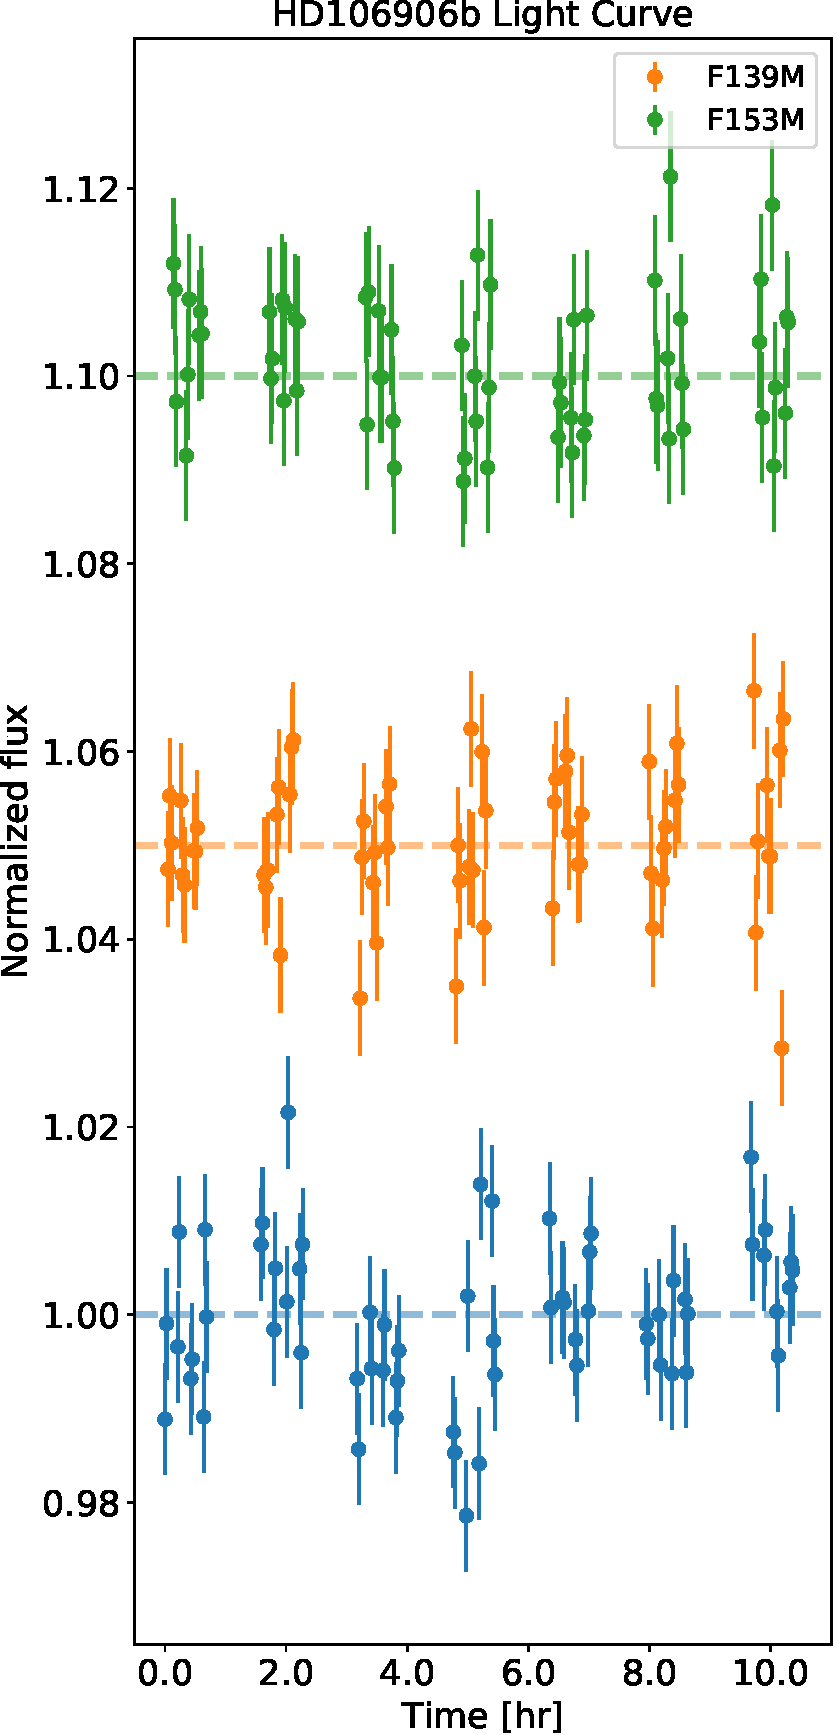
\includegraphics[width=0.5\textwidth]{figures/HD106906_lightcurves.pdf}
  \caption{Light curves for HD106906b in the F127M, F139M, and F153M bands.}
  \label{fig:lightcurve}
\end{figure}

\begin{figure}
  \centering
  \plotone{figures/HD106906_powerspectrum.pdf}
  \plotone{figures/periodogram_bootstrap}
  \caption{Lomb-Scargle periodogram for the light curves of HD106906b. }
  \label{fig:periodogram}
\end{figure}

\begin{figure}
  \centering
  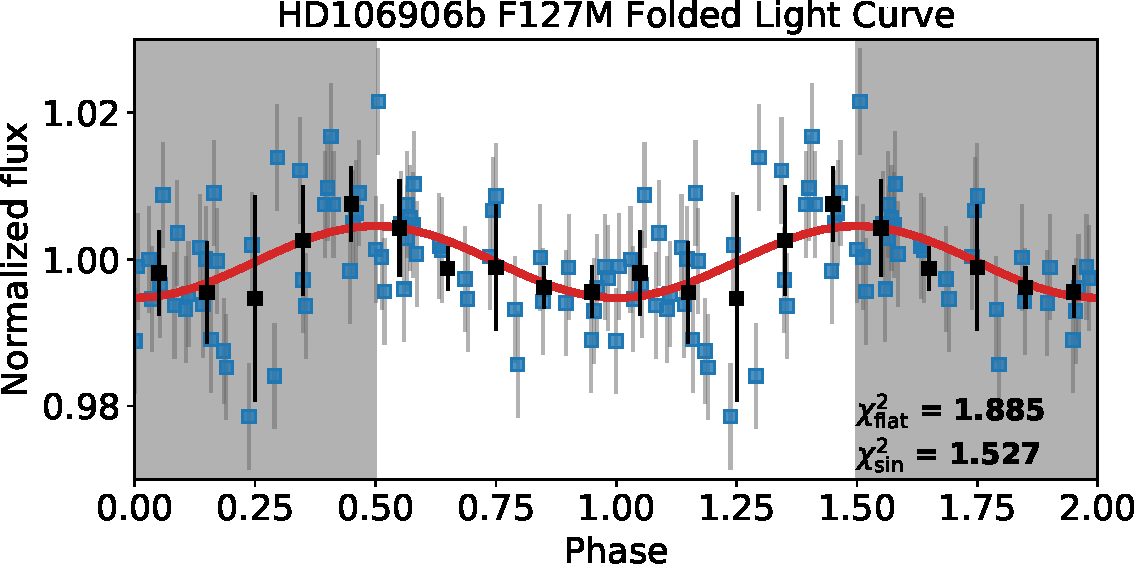
\includegraphics[width=0.5\textwidth]{figures/F127M_foldedLC.pdf}
  \caption{Phase-folded light curve for F127M. The light curve is folded to a period of 4.02 hr. The period corresponds to the most significant peak in the Lomb Scargle periodogram.}
  \label{fig:fold}
\end{figure}

\begin{figure*}
  \centering
    \plotone{figures/all-LSs}
  \caption{Comparison of the periodograms between those for background stars and those for HD106906b. The two background star periodograms that show simialr signals as HD109606b's do not show variations in the folded light curves.}
  \label{fig:all-periodograms}
\end{figure*}


\subsection{Spectral Energy Distribution}
We combine our photometry with archival photometry  to investigate the spectral energy distribution (SED) of HD106906b.  We use HST/ACS/F606W band photometry ($\lambda_{\mathrm{pivot}}=0.596\micron$, FWHM$=0.234\micron$) from \citet{Kalas2015}, $K_{s}$ ($\lambda_{\mathrm{pivot}}=2.145\micron$, FWHM$=0.305\micron$) and $L'$ ($\lambda_{\mathrm{pivot}}=3.774\micron$, FWHM$=0.592\micron$) band photometry from \citet{Bailey2013}. We do not use the archival $J$ band photometry \citep{Wu2016} because our F127M photometry covers similar spectral features and has more than $20\times$ greater SNR. Our F139M photometry provide a tight $1.4\micron$ water absorption constraint for HD106906b.

We fit the SED of HD106906b to the BT Settl model \citep[][]{Allard2012} and show the result in Figure~\ref{fig:SED}. We perform model fitting in magnitude scales, which is the form directly provided by the model.  We convert observed flux intensities to AB magnitudes, and bi-linearly (in \teff and \logg dimension) interpolate the model grid in magnitude scales. The free parameters are effective temperature $\teff$, surface gravity $\logg$, and a scaling parameter $\mathcal{S}$ that is the ratio between the observed flux over model flux. Because model SEDs are presented in flux intensity at the photosphere surface, the scaling parameter can be transformed to the photospheric radius via $R=\sqrt{\mathcal{S}}\,d$ in which $d$ is the distance of the system. Using least $\chi^{2}$ criterion, we find the best-fitting $T_{\mathrm{eff}}=1,800\pm100$~K and $\log g=5.5\pm0.5$.  The scaling parameter corresponds to a radius of  $1.775pm0.015R_{\mathrm{Jup}}$ at a distance of 103.3~pc \citep{Gaia2018,Gaia2016}. The 1,800~K effective temperature estimate is consistent with previous study \citep{Bailey2013,Wu2016}, but the surface gravity is not compatible with a low surface gravity assessment. Additionally, the model SED under-predicts the F139M band flux or over-predicts the depth of the water absorption band (Figure \ref{fig:SED}).

\begin{figure*}
  \centering
  \plottwo{figures/SEDfit.pdf}{figures/SEDfit_zoomin.pdf}
  \caption{The SED of HD106906 and the best-fitting BT Settl model. The left panel shows the full observed SED (blue) that includes photometry from both this observation and archival data. The red line is the best-fitting BT Settl spectrum (1800~K, $\log g=5.5$). The red dots are the model photometry that are from model spectrum integrated with the filter throughput curves. The right panel zooms in the wavelength range of this observation. The orange violin plot shows the uncertainty of the model fitting. The flux in the F139M band is significantly under-predicted by the BT Settl model.}
  \label{fig:SED}
\end{figure*}

\subsection{Astrometry}
\label{sec:astrometry}

We measure the RA and DEC of 16 sources that are in the FoV of both HST/WFC3 epochs. The average uncertainties in RA/DEC are 5.3 mas for the 2016 epoch and 2.9 mas for the 2018 epoch corresponding to 0.041 and 0.023 pixel, respectively. Due to saturation at the PSF core, HD106906A has one of the worst astrometric precisions among all sources. Especially in the 2016 epoch, its RA and DEC combined astrometric uncertainty is 51.2 mas or 0.39 pixel. Astrometric measurements for HD106906 are listed in Table \ref{tab:astrometry} and those for the background sources are listed in Table \ref{tab:bck} in the appendix.

We derive the separations and position angles between HD106906A and b and their uncertainties for the 2016 and 2018 epochs. The separations are $7.11\pm0.03$ and $7.108\pm0.005$ in the 2016 and 2018 epochs, respectively. The position angles are $307.5^{\circ}\pm0.3^{\circ}$ and $307.29\pm0.05^{{\circ}}$ in the two epochs, respectively. These separations and position angles are indistinguishable with those measured in the ACS/HRC images \citep{Bailey2013}. Therefore, relative motions between the companion and the star are not detected. The substantial positional uncertainty of HD106906A due to saturation is the bottleneck that limits the astrometric performance of these HST images.

 \begin{deluxetable}{llclc}
  \tablenum{1}
  \tablecaption{HST/WFC3 Astrometry for HD106906 System.\label{tab:astrometry}}
  
  \tablehead{
    \colhead{Object (epoch)} &
    \colhead{RA} &
    \colhead{$\delta$RA} &
    \colhead{DEC} &
    \colhead{$\delta$DEC}\\
    \colhead{} &
    \colhead{hh mm ss} &
    \colhead{mas} &
    \colhead{dd mm ss} &
    \colhead{mas} 
  }
  
  \startdata
  HD106906A (2016) & 12 17 53.120 & 16 & -55 58 32.158 & 49 \\
  HD106906b (2016) & 12 17 52.4476 & 1.1 & -55 58 27.8270 & 0.79 \\
  HD106906A (2018) & 12 17 53.111 & 5.6 & -55 58 32.157 & 6.7 \\
  HD106906b (2018) & 12 17 52.4376 & 2.1 & -55 58 27.840 & 2.3 \\
  \enddata
\end{deluxetable}

\subsection{Other Sources in the Field of View}
By median combining the entire time series, we construct $33\arcsec\times33\arcsec$ FoV deep images (Figure \ref{fig:2rdi}). These images may include yet undiscovered companions of HD106906. With our observation setups, the water absorption depth can be an effective criterion for selecting ultra-cool objects. Here we define the absolute water absorption depth as the difference between the F139M flux intensity and the continuum, which is the average flux intensity of F127M and F153M. We further define the normalized water absorption depth ($\mathcal{D}$) as the absolute depth divided by the continuum flux intensity. $\mathcal{D}$ is calculated as
\begin{equation}
\mathcal{D} = \frac{(f_{\mathrm{F127M}} + f_\mathrm{F153M})/2 - f_{\mathrm{F139M}}}{(f_{\mathrm{F127M}} + f_\mathrm{{F153M}})/2}
\end{equation}

We calculate the 5-$\sigma$ contrast curves for the median-combined primary-subtracted images in all three bands (Figure \ref{fig:contrast_curve}). The method of constructing these contrast curves through a PSF injection-and-recovery process, which is detailed in  \citet{Zhou2019}.  We find that the three bands  have almost the same contrast curves although the F127M image has deepest the contrast at large separation.  Our median-combined, primary-subtracted images are sensitive to $\Delta \mbox{mag}=7.7$ at 1\arcsec, $\Delta \mbox{mag}=10.4$ at 2\arcsec, and $\Delta \mbox{mag}=14.2$ at 5\arcsec. Assuming an age of 15 Myr and evolution track of \citet{Saumon2008}, our median-combined, primary-subtracted images can place 5-$\sigma$ upper limits for companions more massive than 7\mjup at 2\arcsec or wider and 2\mjup at 4.75\arcsec or wider.

\begin{figure}
  \centering
  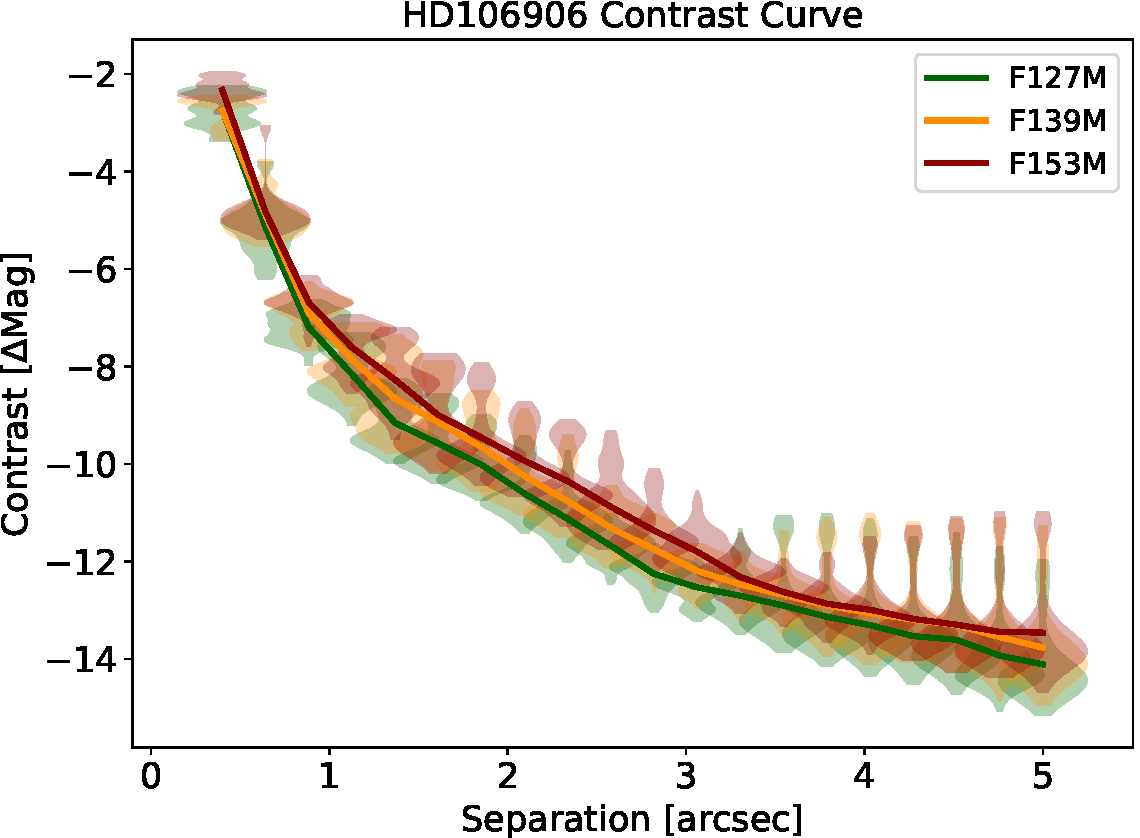
\includegraphics[width=0.5\textwidth]{figures/contrast_curve.pdf}
  \caption{Contrast curves in F127M, F139M, and F153M for the HD106906 observations.}
  \label{fig:contrast_curve}
\end{figure}

We used the median-combined primary-subtracted image to measure the relative water absorption depth for 12 point sources (include HD106906b) that are in the field of view for both telescope rolls. Figure~\ref{fig:backgroundsources} shows the water absorption depth for each source. Except for HD106906b, there is one source that has significant water absorption depth. Interestingly, this source  has the smallest angular separation (0.87\arcsec) to HD106906b among all sources in the field of view.  Based on HST/ACS/HRC and HST/WFC3/IR observation, the spectral energy distribution of this source is best fit to a $3.7\pm0.1\times10^{3}$~K stellar SED model. Therefore, this object is most likely a background K/M giant star.

\begin{figure}
  \centering
  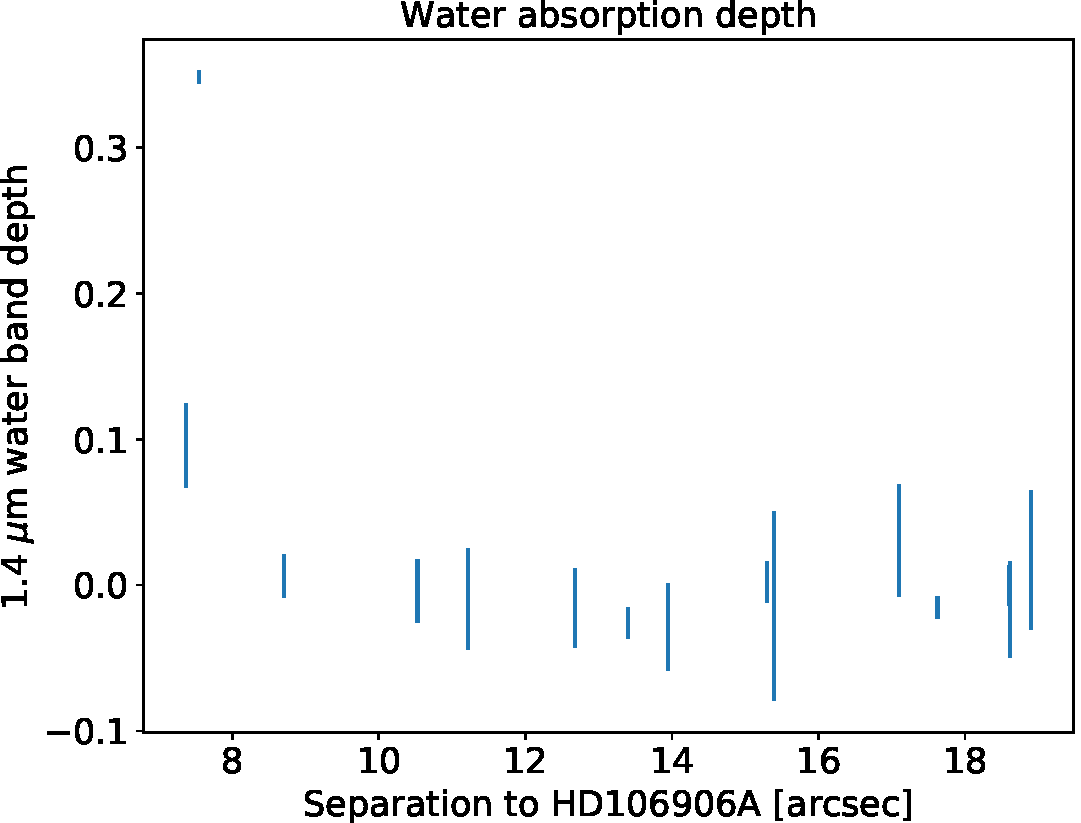
\includegraphics[width=0.5\textwidth]{figures/bck_waterdepth.pdf}
  \caption{Water absorption depths of all sources in the field of view. The sources are ranked by their angular distance to HD106906AB. The two sources (one is HD106906b) that have significant water absorption are also the two that are closest to HD106906AB in agnular distance.}
  \label{fig:backgroundsources}
\end{figure}

We investigate the astrometry of this close companion source, and we particularly caution if this source can contaminate previous observations.  We calculate the differences in right ascension ($\Delta$RA),  declination ($\Delta$DEC), and the separations between HD106906b and the close companion source from the year 2003 (one year before the first direct imaging record of HD106906b) to the year 2023. In this calculation, the close companion is assumed to be stationary and HD106906b is co-moving with its host star at $(\mu_\alpha\cos\delta=-39.01 \mbox{mas/yr}, \mu_{\delta}=-12.87 \mbox{mas/yr})$ \citep{Gaia2016, Gaia2018}. The results are shown in Figure~\ref{fig:astrometry:bck}. In the same figures, we also marked the expected positions of the close companion in previous observations \citep{Bailey2013, Wu2016, Lagrange2016, Daemgen2017} with the stationary background object assumption.

Figure~\ref{fig:astrometry:bck} demonstrates that HD106906b, due to its proper motion, should shorten its separation to the assumed background object the  over the years. The separation between HD1006906b and the assumed background object has been decreasing from 1\arcsec.29 (2004, first imaging record) to 0\arcsec.87 (this study). In the study of \citep{Bailey2013, Wu2016, Daemgen2017}, the HD106906b should have separation of 0.95-1.05 to the close companion, assuming it is stationary. Given their separations in these studies, it is unclear if the background star contaminated those measurements. Considering the brightness contrast of the two objects, in the worst case, the contamination of the background star to HD106906b's broadband photometry is  $<7.5\%$ in the near-infrared. This source is detectable in all three HST observations. HST astrometry of this source agrees with the assumption that it is a stationary background source.

\begin{figure*}
  \centering
  \plottwo{figures/bckStarDeltaRADEC.pdf}{figures/bckStarSeparation.pdf}
  \caption{Relative astrometry between HD106906b and a closeby background star. Left: The difference in right ascension and declination. Right: The separation as a function of time. Past observations of HD106906b are marked as squares.}
  \label{fig:astrometry:bck}
\end{figure*}

% \subsection{Astrometry -- relative to the background star}
% \label{sec:astrometry}



% \Interestingly{Large scale structures}


\section{Discussion}
\subsection{Light curve periodicity}

We evaluate the modulation significance from both instrumental and astrophysical perspective. From the instrumental point of view, we have two arguments against that the modulation signal we see in HD106906b's F127M light curve is due to systematics. First, the F127M, F139M, and F153M observations were taken \emph{de facto} simultaneously. Systematics that introduces periodic/sinusoidal signals at 4 hr timescale in the F127M light curve should have a similar effect on the other two light curves. The agreement of the  F139M and F153M light curves with flat lines is inconsistent with modulation in the F127M light curve being systematics. Second, similar modulations do not appear in the light curves of background stars. We measure and analysis light curves of fifteen brightest background stars that are in the field of view of both telescope roll angles and are not affected by the diffraction spikes of the primary PSFs.
Figure \ref{fig:all-periodograms} shows the comparison between the periodograms of the background stars and that for F127M light curve of HD106906b. Most periodograms of the background star do not show significant signals except one object. However, when we fold its light curve to the period with the most significant peak, the folded light curve is consistent with a flat line. These two lines of evidence argue that systematics is not likely to be the cause of the modulation signal.

From the astrophysical perspective, we evaluate the likelihood for HD106906b to be rotationally modulated only in the F127M band but not the other two bands. Multi-wavelength and time-resolved observations of ultra-cool dwarfs have found the rotational modulations for majority  brown dwarfs and planetary mass companions are wavelength-dependent and have higher amplitude at shorter wavelengths than longer wavelengths \citep[e.g.,][]{Zhou2019,Zhou2016,Yang2014,Apai2013,Schlawin}. This phenomenon is consistent with a theoretical estimate based on Mie-scattering calculation\citep{Schlawin,Hiranaka2016}. Besides, the 1.4 \micron{} water absorption/F139M band often show damped rotational modulation, due to water vapor opacity elevating the photosphere at this wavelength.  Therefore rotational modulation only appearing in the band with the shortest wavelength of our observation is qualitatively consistent with models and previous observations, particularly those for planetary mass companions \citep{Zhou2016,Zhou2019}. If we assume that the wavelength dependence of HD106906b's rotational modulation is the same as that measured in 2M1207b \citep{Zhou2016}, as 2M1207b is the closest analog that also has modulation detected, we expect that the modulation amplitude in the F153M band to be 0.6\%. Our observation is not sensitive to such small amplitude modulations. Therefore, if the overall modulation amplitude is low, it is likely that the signal is only detected in the bluest band of the observation.

These two lines of evidence support the modulation we see in HD106906b's F127M light curve to be astrophysical, in particular, caused by heterogeneous clouds. Nevertheless, we emphasize that the amplitude of the signal is marginal and not significant. Our evaluation of the rotational modulation and rotation period for HD106906b remain inconclusive.


\subsection{SED of  HD106906b}
Two issues have emerged in the SED fitting results. First, the best-fitting model over-predicts the 1.4 \micron{} water absorption band depth. Second, the best-fitting surface gravity is inconsistent with previous low-gravity assessment for HD106906b.

To investigate the first issue, we calculate the water band absorption depths in the BT Settl as functions of $T_{\mathrm{eff}}$ and $\log g$ and compare them with the observed value. As shown in Figure \ref{fig:waterdepth}), for a fixed $T_{\mathrm{eff}}$ of 1800 K, all BT Settl models over-predict the water band depth regardless of \logg. For a fixed $\log g$ of 5.5, to match the observed water band depth, $T_{\mathrm{eff}}$ needs to be raised to $2500$ K, although such a high temperature is not at all consistent with the overall SED shape. Therefore, the mismatch between the HD106906b's observed and the model SEDs in the 1.4 \micron{} water bands demonstrates the inadequacy of current state-of-the-art ultra-cool atmospheric models.

\citet{Bailey2013} and \citet{Daemgen2017} have discussed the surface gravity of HD106906b. Both studies classify HD106906b as a low-to-intermediate surface gravity object based on its triangle-shaped $H$ band spectrum. The equivalent widths of the K I absorption lines measured in \citet{Daemgen2017} are also consistent with an intermediate surface gravity classification. In addition, low surface gravity is also consistent with the young and low mass nature of HD106906b. However, our SED fitting yield a very high gravity result. With a fixed $T_{\mathrm{eff}}$ of 1800 K, lower surface gravity models significantly over-predicts the F153M and $K_{\mathrm{s}}$ band flux intensities. Therefore they are not preferred by the SED fitting. This inconsistency, again, may show the insufficiency of atmospheric models for planetary-mass ultra-cool objects.

\begin{figure}
  \centering
  \plotone{figures/logg_water}
  \plotone{figures/Teff_water}
  \caption{1.4 \micron{} water band depths predicted by the BT Settl model. Left: With a fixed $T_{\mathrm{eff}}=1800$ K, models with $\log g$ between 3 to 5.5 all over-predicts the water band depths. Right: With a fixed $\log g=5.5$, it requires $T_{\mathrm{eff}}=2500$ K for the model to match the observation.}
  \label{fig:waterdepth}
\end{figure}

\subsection{Astrometric Constraints of the  HD106906 system}

With a temporal baseline of 14 years, three epochs HST observations are not able to detect relative motion between HD106906b and its host star. Assuming a face-on, circular orbit with a radius of 732 au, we expect an orbit arc for HD106906b to be 37.1 mas in 14 yr or 5 mas in 2 yr (between the two WFC3 epochs). These arc lengths correspond to $12.8\times$ and $1.72\times$ the average $1$-$\sigma$ astrometric uncertainty in the 2018 epoch. Therefore, HST images can resolve these orbital motion if their precisions are not limited by saturation.

Astrometric constraints of the HD106906 system are critical for studying the system's formation and dynamical evolution history \citep[e.g., ][]{DeRosa2019} and measuring the dynamical mass of the planet \citep[e.g.,][]{Snellen2018,Dupuy2019}. Design of future observations should consider optimization for astrometric precisions, such as avoiding saturation and increasing spatial resolution through dithering. In the $33\times33$ arcsec$^{2}$ FoV of WFC3 images, there are seven background sources that have sky coordinate and proper motion measurements from GAIA. Using these sources to register the WFC3 image with GAIA can calibrate the absolute astrometry to sub-mas precision level \cite{Bedin2018}. Future astrometric analysis of HD106906 system will be benefited from our background source catalog.

\section{Conclusion}

\begin{enumerate}
\item We observed planetary mass companion HD106906b with seven contiguous HST orbits in HST WFC3/IR direct-imaging mode. We have achieved nearly photon-noise limited  light curves in F127M, F139M, and F153M bands. Rotational modulations marginally ($2-\sigma$) present in the F127M band but are absent in the other two bands.

\item Comparing to planetary mass companions that have time-resolved observations, the marginal detection of  F127M band modulations and non-detections in other two bands are consistent with those observed in brown dwarfs and planetary mass companions, for which the rotational modulations are detected at high significance. The wavelength-dependent rotational modulations are consistent with the interpretation that the modulations are caused by heterogeneous condensate clouds.

\item Our observations provide the first 1.4 \micron water band photometry for HD106906b. We combine our three bands of photometry with archival data to form a SED for HD106906b and perform SED model fitting. We find a best-fitting effective temperature of 1800~K, consistent with literature results, and a best-fitting surface gravity $\log g$ of 5.5,  significantly higher than previous estimates and inconsistent with HD106906b being a young and planetary mass object. Also, the observed F139M band flux intensity for HD106906b is significantly higher than the best-fitting model value. These inconsistencies may suggest inadequacies of the BT-Settl model for young planetary mass objects.

\item We combine WFC3/IR images to form primary-subtracted deep images and search for planetary mass companions in the FoV. Our composite images are sensitive to a planet with a mass of $\sim 2 \mjup$. We used the 1.4mm water absorption to vet the close companions. We did not discover  any new companions. We did find a point source that has a lower flux in the F139M band. This object is likely a background K/M giant based on astrometric and SED analysis.  Based on GAIA astrometry and proper motion, the angular distance between HD106906b and its closest apparent companion is decreasing and will be on the level of 0.7\arcsec-0.8\arcsec  in the 2020s decade. Future observations of HD106906b needs to eliminate contamination from the close companion carefully.

\item We measured astrometry for HD106906 A and b, as well as the background sources. The separation and position angle between HD106906 A and b in the 2016 and 2018 epochs WFC3 images are consistent with those in the 2004 ACS/HRC images within 1-$\sigma$ errorbar. Relative motion between HD106906 A and b is not detected. 
\end{enumerate}
% \end{enumerate}
% For the last point, take the variability occurrence rate from \citep{Vos2017,Metchev2015}, test whether the low mass companions' variability occurrence rate agree with the low surface gravity field objects

\clearpage
\appendix
\section{Background source information}
Table \ref{tab:bck} summarizes the information for background sources.
\begin{deluxetable*}{cccccc}
  \tablenum{2}
  \tablecaption{Background Sources in the Field of View\label{tab:bck}}
  
  \tablehead{
    \colhead{Source ID} &
    \colhead{RA} &
    \colhead{DEC} &
    \colhead{Flux$_{\mathrm{F127M}}$} &
    \colhead{Flux$_{\mathrm{F139M}}$} &
    \colhead{Flux$_{\mathrm{F153M}}$} \\
    \colhead{} &
    \colhead{hh mm ss} &
    \colhead{dd mm ss} &
    \colhead{\fluxunit} &
    \colhead{\fluxunit} &
    \colhead{\fluxunit} 
  }
  
  \startdata
cc01 & $184 28 22.332$ & $-55 58 13.65$    & 1.91e-17 & 1.68e-17 & 1.49e-17\\
cc02 & $184 28 20.004$ & $-55 58 18.743$   & 1.76e-17 & 1.58e-17 & 1.33e-17\\
cc03 & $184 28 19.341$ & $-55 58 19.44$    & 3.43e-18 & 3.22e-18 & 2.93e-18\\
cc04 & $184 28 23.742$ & $-55 58 18.544$   & 3.48e-18 & 3.25e-18 & 2.83e-18\\
cc05 & $184 28 12.5235$ & $-55 58 17.057$  & 1.12e-17 & 9.91e-18 & 8.39e-18\\
cc06 & $184 28 02.9175$ & $-55 58 23.99$   & 2.96e-17 & 2.62e-17 & 2.22e-17\\
cc07 & $184 28 06.798$ & $-55 58 23.506$   & 5.58e-18 & 4.93e-18 & 4.24e-18\\
cc08 & $184 28 08.016$ & $-55 58 25.292$   & 1.11e-17 & 9.68e-18 & 8.70e-18\\
cc09 & $184 28 06.054$ & $-55 58 28.655$   & 4.22e-18 & 3.35e-18 & 3.37e-18\\
cc10 & $184 27 46.2585$ & $-55 58 32.879$  & 2.72e-16 & 2.44e-16 & 2.08e-16\\
cc11 & $184 28 34.815$ & $-55 58 26.229$   & 2.94e-18 & 2.61e-18 & 2.46e-18\\
cc12 & $184 28 18.6075$ & $-55 58 13.471$  & 2.66e-18 & 2.39e-18 & 2.21e-18\\
cc13 & $184 28 05.4135$ & $-55 58 16.422$  & 2.11e-18 & 1.84e-18 & 1.71e-18\\
cc14 & $184 27 59.292$ & $-55 58 16.23$    & 1.70e-18 & 1.53e-18 & 1.41e-18\\
cc15 & $184 28 02.337$ & $-55 58 19.313$   & 1.17e-18 & 1.05e-18 & 8.63e-19\\
  \enddata
\end{deluxetable*}
\bibliographystyle{yahapj}
\bibliography{library}
\end{document}
%%% Local Variables:
%%% mode: latex
%%% TeX-master: t
%%% End:

% LocalWords:  AAS
